\documentclass[11pt,a4paper]{article}
\usepackage{pgcomprt}
\usepackage{graphicx}
\usepackage[utf8]{inputenc}
% \usepackage[portuges,brazilian]{babel}
\usepackage{lipsum}
%\usepackage[dvipdfm]{hyperref}
\usepackage[colorinlistoftodos]{todonotes}
\usepackage{tabularx}
\usepackage{caption}
\usepackage{multirow}
\usepackage{blindtext}
\usepackage{multicol}

% glossary
\usepackage{glossaries} 
\newglossaryentry{domain-knowledge}{%
  name={domain knowledge},%
  description={valid knowledge used to refer to an area of human endeavour, an autonomous computer activity, or other specialized discipline}}

\newacronym{tla}{TLA}{Three Letter Acronym}
\makeglossaries

\begin{document}

%% Preenchimento dos parâmetros do PGCOMP
\TextoPortugues{true} % 'true' para português, 'false' para inglês 
\PGCOMPSeqAno{100/2014}  % Número e ano(YY) da MCC
\TituloCapa{Arquitetura de Software do Projeto MIDAS 1.6}
\TituloRosto{Arquitetura de Software do Projeto MIDAS 1.6}
\MesTexto{Abril} % Mês por extenso, em português ou inglês
\AnoYYYY{2017}   % Ano com 4 digitos
\QtdLinhasTituloCapa{2} % Qtd de linhas do titulo na capa, de 1 até 4 linhas

\QtdAutores{9} % Define quantidade de autores: 1, 2, ou 3
%%%% Dados Autor 1 %%%%%%%%%%%%%%%%%%%%%%%%%%%%%%%%%%%%%%%%
\AutorANome{Daniel Moreira}
\AutorAemail{danieltimponi@ufba.br}
\AutorADI{true} % 'true' se o autor for do DI
\AutorAinst{ % Instituição do autor, caso não seja do DI
}
%%%% Dados Autor 2 %%%%%%%%%%%%%%%%%%%%%%%%%%%%%%%%%%%%%%%%
\AutorBNome{Juvenal Macêdo}
\AutorBemail{juniormacedovc@gmail.com}
\AutorBDI{true} % 'true' se o autor for do DI
\AutorBinst{ % Instituição do autor, caso não seja do DI
}
%%%% Dados Autor 3 %%%%%%%%%%%%%%%%%%%%%%%%%%%%%%%%%%%%%%%%
\AutorCNome{Leila Anjos}
\AutorCemail{lkarita@gmail.com}
\AutorCDI{true} % 'true' se o autor for do DI
\AutorCinst{ % Instituição do autor, caso não seja do DI
}
%%%% Dados Autor 4 %%%%%%%%%%%%%%%%%%%%%%%%%%%%%%%%%%%%%%%%
\AutorINome{Lucas Cardoso}
\AutorIemail{kardoso@gmail.com}
\AutorIDI{true} % 'true' se o autor for do DI
\AutorIinst{ % Instituição do autor, caso não seja do DI
}

%%%% Dados Autor 4  %%%%%%%%%%%%%%%%%%%%%%%%%%%%%%%%%%%%%%%%
\AutorDNome{Marco Paranhos}
\AutorDemail{marco.paranhos1@gmail.com}
\AutorDDI{true} % 'true' se o autor for do DI
\AutorDinst{ % Instituição do autor, caso não seja do DI
}
%%%% Dados Autor 5 %%%%%%%%%%%%%%%%%%%%%%%%%%%%%%%%%%%%%%%%
\AutorENome{Moara Brito}
\AutorEemail{moarabritto@gmail.com}
\AutorEDI{true} % 'true' se o autor for do DI
\AutorEinst{ % Instituição do autor, caso não seja do DI
}
%%%% Dados Autor 6  %%%%%%%%%%%%%%%%%%%%%%%%%%%%%%%%%%%%%%%%
\AutorFNome{Neyla Fontan}
\AutorFemail{neylafontan@gmail.com}
\AutorFDI{true} % 'true' se o autor for do DI
\AutorFinst{ % Instituição do autor, caso não seja do DI
}
%%%% Dados Autor 7d%%%%%%%%%%%%%%%%%%%%%%%%%%%%%%%%%%%%%%%%
\AutorGNome{Ricardo Teixeira}
\AutorGemail{ricardo.btxr@gmail.com}
\AutorGDI{true} % 'true' se o autor for do DI
\AutorGinst{ % Instituição do autor, caso não seja do DI
}
%%%% Dados Autor 8  %%%%%%%%%%%%%%%%%%%%%%%%%%%%%%%%%%%%%%%%
\AutorHNome{João Werther}
\AutorHemail{jwertherf@gmail.com}
\AutorHDI{true} % 'true' se o autor for do DI
\AutorHinst{ % Instituição do autor, caso não seja do DI
}

\PatrocinioFlag{false} % 'true' para incluir nota de rodapé da folha de rosto
\Patrocinio{ % Texto da nota de rodapé para patrocínio
Trabalho patrocinado pelo Ministério de Ciência e Tecnologia da Presidência da República Federativa do Brasil 
(e agência de fomento e o número do processo, se aplicável). (Ou em Inglês: This work has been
sponsored by the Ministério de Ciência e Tecnologia da Presidência da República
Federativa do Brasil.
}


\Resumo{  % Resumo em Português. Para Trabalho em Português
\textbf{Resumo: }Este relatório técnico foi elaborado em atendimento à tarefa definida como trabalho final da disciplina  MATE67 - Arquitetura de Software, do Programa de Pós-Graduação em Ciência da Computação da Universidade Federal da Bahia, sob orientação da professora Christina Von Flach Garcia Chavez. O documento foi produzido pela equipe de alunos que ficou responsável por estudar e documentar a arquitetura de software do projeto MIDAS, que é uma proposta de solução de \textit{middleware} para interoperabilidade entre nuvens. Este trabalho visa  propiciar aos alunos que cursaram a disciplina a oportunidade de aplicar na prática os conhecimentos teóricos adquiridos  em um \textit{case} de projeto real. Adicionalmente, o conteúdo deste documento poderá ser incorporado à tese de doutorado sobre o MIDAS como representação das decisões arquiteturais propostas pela equipe do projeto.


}

%\PalavrasChave{ }

%\Abstract{}
%\Keyword{}



% Comando para geração da Capa
\Capa

% Comando para geração da Fohas de Rosto
\FolhaRosto


\section*{Glossário}
\begin{description}
\item[API] \textit{Application Programming Interface}
\item[C\&C] Componente e Conector
\item[CSV] \textit{Comma-separated values}
\item[DaaS] \textit{Data as a Service}
\item[DIS] \textit{Dataset Information Storage}
\item[IaaS] \textit{Infrastructure as a Service}
\item[JSON] \textit{JavaScript Object Notation}
\item[PaaS]\textit{Platform as a Service}
\item[PHP]\textit{Hypertext Preprocessor}
\item[REST]\textit{Representational State Transfer }
\item[SaaS] \textit{Software as a Service}
\item[SEI] \textit{Software Engineering Institute}
\item[XML] \textit{eXtensible Markup Language}
\item[WBS] \textit{Work breakdown structure}

\end{description}
\newpage

% TABLE OF CONTENTS -  OPTIONAL
\Sumario{3} % Gera índice com profundidade x

%%%%%%%%%%%%%%%%%%%%%%%%%%%%%
%%                                                     %%
%%          BEGIN DOCUMENT               %%
%%                                                     %%
%%%%%%%%%%%%%%%%%%%%%%%%%%%%%

\section{Apresentação geral do documento}

Este relatório possui como propósito documentar as etapas de Análise de Requisitos de  Software e Projeto de Arquitetura de Software do MIDAS, versão 1.6. Os processos seguidos nestas duas etapas são apresentados na Figura~\ref{fig:visaogeral}. 
\todo{Esta figura é uma sugestão dos processos que seguimos}
\begin{figure} [h!]
  \centering
    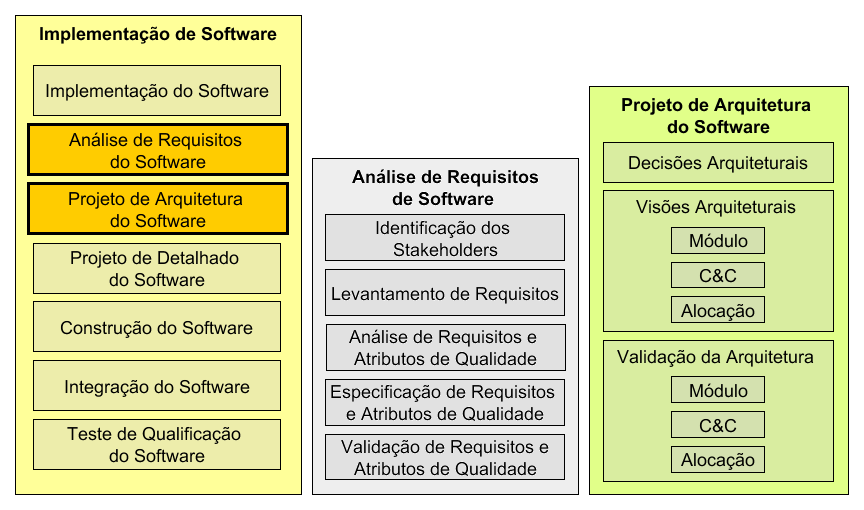
\includegraphics[width=0.9\textwidth]{visaogeral}
  \caption{Grupos de fluxo de processos de software}
  \label{fig:visaogeral}
\end{figure}

Na etapa de Análise de Requisitos, apresentado na Seção~\ref{sec:analise}, visou-se definir os requisitos de software funcionais e não funcionais seguindo as recomendações do padrão internacional ISO/IEC 12207~\cite{ISOIEC21207}. Os atributos de qualidade foram estabelecidos seguindo o modelo de qualidade recomendado pelo padrão internacional ISO/IEC 9126-1:2001~\cite{ISOIEC9126}. Como saída desta etapa, obteve-se os seguintes artefatos:\todo {estranho artefatos}

\begin{enumerate}
\item Lista de \textit{stakeholders}, Subseção~\ref{subsec:stakeholders};
\item Requisitos arquiteturais, Subseção~\ref{subsec:ra};
\item Atributos de qualidade, Subseção~\ref{subsec:aq}.
\end{enumerate}

% ISO 12207 Requisitos
% The purpose of Software Requirements Analysis Process is to establish the requirements of the software elements of the system.

% ISO 9126-1 Qualidade interna e externa

% ISO12207 Arquitetura
% The purpose of the Software Architectural Design Process is to provide a design for the software that implements and can be verified against the requirements.

%No sentido de capturar as várias dimensões de um projeto arquitetural, o documento é estruturado de acordo com Germoglio  \cite{germoglio2010arquitetura} e Clements et al \cite{clements2002documenting}.

\todo{Pt ou En?}
A etapa Projeto de Arquitetura de Software, Seção~\ref{sec:pas}, tem como objetivo fornecer um modelo arquitetural para o MIDAS, que seja capaz de ser implementado e validado de acordo com os requisitos de software definidos. Para construção do modelo arquitetural, utilizou-se as três visões arquiteturais propostas pelo \textit{Software Engineering Institute} (SEI)~\cite{clements2002documenting}, que devem ser especializadas por um estilo arquitetural. Como resultado desta etapa, elaborou-se as visões arquiteturais do MIDAS:

\begin{multicols}{2}
\begin{enumerate}
\item Módulo, Subseção~\ref{subsec:mv}:
	\begin{itemize}
	\item[-] \textit{Decomposition Style}; 
    \item[-] \textit{Data Model Style};
    \item[-] \textit{Uses Style};
    \item[-] \textit{Layered Style}.
	\end{itemize}
\item Componente e Conector, Subseção~\ref{subsec:cc}
	\begin{itemize}
	\item[-] Estilo cliente-servidor.
	\end{itemize}
\item Alocação, Subseção~\ref{subsec:av}
	\begin{itemize}
	\item[-] \textit{Deployment Style}; 
    \item[-] \textit{Work Assignment Style}.
	\end{itemize}
\end{enumerate}

\end{multicols}

%Baseado em Germoglio \cite{germoglio2010arquitetura} é apresentado os requisitos arquiteturais que são os requisitos que possui relevância para a arquitetura, os \textit{stakeholders} que são os participantes do projeto, os atributos de qualidades, e as decisões arquiteturais que são as escolhas entre as alternativas de design arquitetural.

%Clements et al \cite{clements2002documenting} apresenta três \textit{view types}, e estas serão representadas neste documento. O \textit{Module View} fornece a decomposição em unidades de implementação do sistema,  com isso será representado o \textit{Decomposition Style}, o \textit{Data Model Style}, o \textit{Uses Style} que ilustra a depêndencia que pode existir entre dois módulos, e o \textit{Layered Style}.
%O \textit{Component-and-Connector View} expressam o comportamento de tempo de execução e neste documento é representado pelo \textit{Client-Server Style}
%A \textit{Allocation View} descreve o mapeamento de unidades de software para elementos de um ambiente no qual o software é desenvolvido ou executado. Dessa forma, o \textit{Deployment Style} representa a implantação da aplicação no hardware, e o  \textit{Work Assignment Style} descreve o mapeamento das pessoas no desenvolvimento do MIDAS.

%Não fez parte do escopo deste trabalho alterar ou interferir em  decisões arquiteturais do projeto. O trabalho da equipe restringiu-se a documentar as decisões arquiteturais da versão 1.6 previamente estabelecidas pela equipe que participa do MIDAS.   





\newpage

\section{Finalidade do sistema}

O MIDAS visa atender a interoperabilidade de serviços entre nuvens, onde tem por objetivo estabelecer uma comunicação transparente entre aplicações do tipo \textit{Software as a Service }(SaaS) e dados de quaisquer provedores de Dado como Serviço (DaaS), de forma que as aplicações possam trabalhar com conjuntos de dados de serviços DaaS de qualquer fonte. O MIDAS converte a consulta original para uma requisição DaaS adequada e a envia para o provedor do serviço. O resultado obtido é então formatado de acordo com a resposta esperada pela aplicação \cite{marinho2016midas}.

O  projeto MIDAS é conduzido pelo Departamento de Ciência da Computação da Universidade Federal da Bahia sob orientação da professora Daniela Claro e conta com a participação de alunos de doutorado, mestrado e graduação da universidade.

\todo[inline]{adicionar ao texto}
A Tabela~\ref{tab:problema} apresenta-se informações do domínio de aplicação e as funcionalidades, serviços e restrições do sistema.  

\begin{table}[h]
\centering
\caption{Definição do problema} \label{tab:problema}
\begin{tabular*}{\linewidth}{@{\extracolsep{\fill}}|r p{10.9cm}|} \hline
\textbf{Domínio} & Computação em nuvem.  \\ \hline
\textbf{Problema} & Baixa interoperabilidade entre nuvens.  \\\hline
\textbf{Consequência} & Os usuários finais buscam por conteúdos em diferentes provedores DaaS e como consequência os desenvolvedores de aplicações da camada SaaS têm trabalho extra para adaptar suas aplicações a diferentes provedores DaaS.
  \\\hline
\textbf{Proposta} & Introdução de um \textit{middleware} para aumentar a interoperabilidade entre as camadas SaaS e DaaS.  \\\hline
\end{tabular*}
\end{table}




%%%%%%%%%%%%%%%%%%%%%%%%%%%%%%%%%%%
%%%%%%%%%%%%%%%%%%%%%%%%%%%%%%%%%%%
%%%%%%%%%%%%%%%%%%%%%%%%%%%%%%%%%%%
%%%%%%%%%%%%%%%%%%%%%%%%%%%%%%%%%%%
\newpage
\section{Análise de requisitos de software}
\label{sec:analise}
Os processos utilizados para realização da análise de requisitos do MIDAS são mostrados na Figura~\ref{fig:analisereq}. 
O levantamento de requisitos foi feito por meio do estudo da documentação existente referente ao MIDAS~\cite{monovini2015,monotarcio2015,marinho2016midas,apresentacao2017} e de uma entrevista com desenvolvedores do MIDAS.
Os requisitos e atributos de qualidade apresentados nesta seção foram validados pelos desenvolvedores e arquitetos de software da equipe MIDAS.  

\begin{figure} [h!]
  \centering
    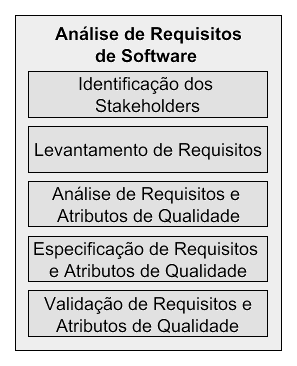
\includegraphics[width=0.32\textwidth]{analisereq}
  \caption{Processos da Análise de Requisitos de Software} 
  \label{fig:analisereq}
\end{figure}



%%%%%%%%%%%%%%%%%%%%%%%%%%%%%%%%%%%
%%%%%%%%%%%%%%%%%%%%%%%%%%%%%%%%%%%
\subsection{\textit{Stakeholders}}
\label{subsec:stakeholders}

\begin{enumerate}
\item \textbf{Usuário final}: o usuário final utiliza a aplicação da camada SaaS para acessar os dados da camada DaaS.
\item 
\textbf{Aplicação \textit{middleware} (MIDAS)}: o \textit{middleware} é responsável por garantir a interoperabilidade na comunicação entre aplicações no camada SaaS e dados na camada DaaS. A equipe do MIDAS pode ser vista na Tabela~\ref{tab:equipe}.
\begin{table}[h]
\centering
\caption{Equipe MIDAS} \label{tab:equipe}
\begin{tabular*}{0.85\linewidth}{@{\extracolsep{\fill}}|r p{7cm}|} \hline
\textbf{Desenvolvedores} & Edmilson Lima, Joevan Santos  \\ \hline
\textbf{ Desenvolvedor de teste} & Marcelo Aires, Witã Rocha, Babacar Mane, Elivaldo Lozer.  \\\hline
\textbf{Arquiteto de software} &Babacar Mane, Marcelo Aires, Elivaldo Lozer, [alunos de MAT65]
  \\\hline
\textbf{Analista de sistema} & Daniel Moreira, Juvenal Macedo
  \\\hline
  \textbf{Fornecedor de requisitos} & Elivaldo Lozer, Marcelo Aires
  \\\hline
  \textbf{Gerente de projeto} & Daniela Claro
  \\\hline
\end{tabular*}
\end{table}
\item \textbf{Provedor DaaS}: o modelo DaaS estabelece regras de acesso ao banco de dados em nuvens. 
\item \textbf{Provedor SaaS}: o SaaS provê serviços de acesso a dados em nuvens ao usuário final. 
%\item \textbf{Aplicação SaaS cliente}: o cliente SaaS utiliza o \textit{middleware} para acessar o banco de dados na camada DaaS. 
%\item \textbf{Banco de dados DaaS}: o banco de dados DaaS fornece os dados requisitados pelo \textit{middleware}. 
\end{enumerate}


%%%%%%%%%%%%%%%%%%%%%%%%%%%%%%%%%%%%%%%%%%%%%%
%%%%%%%%%%%%%%%%%%%%%%%%%%%%%%%%%%%%%%%%%%%%%%
%%%%%%%%%%%%%%%%%%%%%%%%%%%%%%%%%%%%%%%%%%%%%%
%%%%%%%%%%%%%%%%%%%%%%%%%%%%%%%%%%%%%%%%%%%%%%
\newpage
\subsection{Requisitos arquiteturais}
\label{subsec:ra}
Neste seção, define-se os requisitos funcionais e não funcionais do MIDAS. O levantamento de requisitos e análise de requisitos foram realizados seguindo recomendações do padrão internacional ISO/IEC 12207~\cite{ISOIEC21207}.  
%chrome-extension://ecnphlgnajanjnkcmbpancdjoidceilk/content/web/viewer.html?file=http%3A%2F%2Fdisi.unal.edu.co%2Fdacursci%2Fsistemasycomputacion%2Fdocs%2FSystemsEng%2FISO_IEC_12270_2008.pdf

%O levantamento de requisitos foi realizado por meio de uma entrevista, onde os fornecedores de requisitos foram entrevistados pelos analistas de sistema. 

%%%%%%%%%%%%%%%%%%%%%%%%%%%%%%%%%%%
%%%%%%%%%%%%%%%%%%%%%%%%%%%%%%%%%%%
%\newpage
\subsection*{Requisitos funcionais}

A Tabela~\ref{tab:rf} apresenta os requisitos funcionais do MIDAS, que descrevem as diversas funções que clientes e usuários querem ou precisam que o software ofereça.

\begin{table}[htb]
\centering
\caption{Requisitos funcionais} \label{tab:rf}
\begin{tabular*}{\linewidth}{@{\extracolsep{\fill}}|r p{13cm}|}    \hline
\textbf{RF01} 	& \textbf{Decompor consultas}\\ \cline{2-2}
 				& O MIDAS deve aceitar consultas no formato SQL e MongoDB. As consultas devem ser decompostas por comandos SQL.  \\\hline
\textbf{RF02} 	& \textbf{Reconstruir consultas}\\ \cline{2-2}
 				& O MIDAS deve reconstruir a consulta decomposta de modo que ela seja compatível com as DaaSs alvo.   \\ \hline
\textbf{RF03} 	& \textbf{Armazenar e gerenciar informações das DaaSs}\\ \cline{2-2}
 				& O MIDAS deve armazenar e gerenciar informações relevantes das DaaSs (informação de conexão, estruturação da consulta, etc.) .  \\ \hline
 \textbf{RF04} 	& \textbf{Formatar, organizar e filtrar o resultado da consulta no DaaS}\\ \cline{2-2}
 				& O MIDAS deve filtrar dados irrelevantes para o SaaS, organizar os dados,  e ser capaz de retornar o resultado da consulta no formato JSON.  \\ \hline
\end{tabular*}
\end{table}
%%%%%%%%%%%%%%%%%%%%%%%%%%%%%%%%%%%
%%%%%%%%%%%%%%%%%%%%%%%%%%%%%%%%%%%
%\newpage
\subsubsection*{Requisitos não funcionais}
A Tabela~\ref{tab:rnf} mostra os requisitos não funcionais do MIDAS, onde é apresentado as qualidades globais que o MIDAS deve possuir. 


\begin{table}[htb]
\centering
\caption{Requisitos não funcionais} \label{tab:rnf}
\begin{tabular*}{\linewidth}{@{\extracolsep{\fill}}|r p{13cm}|} \hline
\textbf{RNF01} & \textbf{Licença}\\ \cline{2-2}
 & Livre  \\\hline
\textbf{RNF02} & \textbf{Linguagem de programação}\\ \cline{2-2}
 & PHP  \\ \hline
\textbf{RNF03} &\textbf{ Protocolo de comunicação SaaS}\\ \cline{2-2}
 & API REST  \\ \hline
 \textbf{RNF04} & \textbf{Protocolo de comunicação DaaS}\\ \cline{2-2}
 & API REST  \\ \hline
 \textbf{RNF05} & \textbf{Ferramentas (PaaS)}\\ \cline{2-2}
 & Apache 2.0, servidor PHP 5.6   \\ \hline
 \textbf{RNF06} & \textbf{Arquitetura multilocatário}\\ \cline{2-2}
 & A arquitetura de rede deve possibilitar acesso de múltiplas aplicações da camada SaaS.  \\ \hline
\end{tabular*}
\end{table}
%%%%%%%%%%%%%%%%%%%%%%%%%%%%%%%%%%%
%%%%%%%%%%%%%%%%%%%%%%%%%%%%%%%%%%%
\newpage
\subsection{Atributos de qualidade}
\label{subsec:aq}
Na Tabela~\ref{tab:aqs} encontra-se os atributos de qualidade do MIDAS, que foram definidos seguindo as especificações do padrão internacional ISO/IEC 9126-1:2001 \cite{ISOIEC9126}.

\begin{table}[htb]
\centering
\caption{Atributos de qualidade internos e externos de software} \label{tab:aqs}
\begin{tabular*}{\linewidth}{@{\extracolsep{\fill}}|r r p{12.5cm}|} \hline

%%%%%%%%%%%%%%%%%%%%%%%
& \multicolumn{2}{l|}{\textbf{Funcionalidade}}  \\ \cline{2-3}

&\textbf{AQ01} & \textbf{\underline{Interoperabilidade} (Interno)}\\ 
& & O \textit{middleware} deve ser capaz de comunicar simultaneamente com mais de um provedor de nuvem, independentemente das diferenças entre os provedores. Assim, o \textit{middleware} deve garantir a interoperabilidade sintática.  \\\cline{2-3}

&\textbf{AQ02} & \textbf{\underline{Segurança} (Interno)}\\
& & Os dados consultados pelo \textit{middleware} são de domínio público e não requerem criptografia.  \\ \cline{1-3}


%%%%%%%%%%%%%%%%%%%%%%%%
 & \multicolumn{2}{l|}{\textbf{Usabilidade}} \\ \cline{2-3}
 
&\textbf{AQ03} & \textbf{\underline{Operabilidade} (Externo)}\\
& & As aplicações SaaS devem ser capazes de utilizar o \textit{middleware} para requerer informações do DaaS.  \\ \cline{1-3}


%%%%%%%%%%%%%%%%%%%%%%%%
 & \multicolumn{2}{l|}{\textbf{Confiabilidade}} \\ \cline{2-3}
 
&\textbf{AQ04} & \textbf{\underline{Disponibilidade} (Externo)}\\ 
& & O \textit{middleware} deve estar sempre disponível para atender as requisições das aplicações do SaaS.  \\ \hline

 

 
%%%%%%%%%%%%%%%%%%%%%%%%%% 
& \multicolumn{2}{l|}{\textbf{Eficiência}} \\ \cline{2-3}

&\textbf{AQ05} & \textbf{\underline{Desempenho} (Interno e externo)}\\ 
& & Os usuários finais não devem perceber atrasos nas respostas devido a introdução do \textit{middleware}.\\&
&\textbf{Monitoramento}: deve-se monitorar o tempo de resposta de cada requisição para garantir a invisibilidade do \textit{middleware} durante os testes.   \\ \hline

%%%%%%%%%%%%%%%%%%%%%%%
& \multicolumn{2}{l|}{\textbf{Manutenibilidade}} \\ \cline{2-3}

&\textbf{AQ06} & \textbf{\underline{Modificabilidade} (Interno)}\\ 
& & Gerenciador de código\textbf{:} o código-fonte deve ser modificado com o auxílio de um software de controle de versões. Os desenvolvedores utilizaram \textit{branches} e o gerente de desenvolvimento deve aprovar as manutenções antes de subir a alteração ao repositório central. \\&
&\textbf{Acoplamento e Coesão}: o sistema deve possuir baixo acoplamento e alta coesão. O objetivo é diminuir propagação de erros e dependências. \\&
&\textbf{Manutenção preditiva}: para cada alteração no código, deve ser previsto unidades que devem ser modificadas em conjunto.  \\ \cline{2-3}
 
&\textbf{AQ07} & \textbf{\underline{Testabilidade} (Interno)}\\ 
& &  Toda e qualquer alteração deve passar testes manuais. \\\cline{1-3}

%%%%%%%%%%%%%%%%%%%%%%
& \multicolumn{2}{l|}{\textbf{Portabilidade}} \\ \cline{2-3}

&\textbf{AQ08} & \textbf{\underline{Adaptabilidade} (Interno)}\\ 
& &  O MIDAS deve ser capaz de comunicar-se com múltiplas aplicações da camada SaaS e diversas bases de dados da camada DaaS. \\\cline{1-3}

\end{tabular*}
\end{table}





%\begin{table}[htb]
%\centering
%\caption{Atributos de qualidade de software} %\label{tab:aqs}
%\begin{tabular*}{\linewidth}{@{\extracolsep{\fill}}|r p{13cm}|} \hline

%\textbf{AQ01} & \textbf{Interoperabilidade}\\ \cline{2-2}
 %& O \textit{middleware} deve ser capaz de comunicar simultaneamente com mais de um provedor de nuvem, independentemente das diferenças entre os provedores. Assim, o \textit{middleware} deve garantir a interoperabilidade sintática.  \\\hline

%\textbf{AQ02} & \textbf{Disponibilidade}\\ \cline{2-2}
% & O \textit{middleware} deve estar sempre disponível para atender as requisições das aplicações do SaaS.  \\ \hline
 
%\textbf{AQ03} & \textbf{Desempenho}\\ \cline{2-2}
 %& Os usuários finais não devem perceber atrasos nas respostas devido a introdução do \textit{middleware}.\\&
%\textbf{Monitoramento}: deve-se monitorar o tempo de resposta de cada requisição para garantir a invisibilidade do \textit{middleware} durante os testes.   \\ \hline

 %\textbf{AQ04} & \textbf{Modificabilidade}\\ \cline{2-2}
% & Gerenciador de código: o código-fonte deve ser modificado com o auxílio de um software de controle de versões. Os desenvolvedores utilizaram \textit{branches} durante a etapa de manutenção e o gerente de desenvolvimento deve aprovar as manutenções antes de subir a alteração ao repositório central. \\&
%\textbf{Testes}: toda e qualquer alteração deve passar testes manuais. \\&
%\textbf{Acoplamento e Coesão}: o sistema deve possuir baixo acoplamento e alta coesão. O objetivo é diminuir propagação de erros e dependência entre unidades. \\&
%\textbf{Manutenção preditiva}: para cada alteração no código, deve ser previsto unidades que devem ser modificadas em conjunto.  \\ \hline

%\textbf{AQ05} & \textbf{Segurança}\\ \cline{2-2}
% & Os dados consultados pelo \textit{middleware} são de domínio público e não requerem criptografia.  \\ \hline
%\end{tabular*}
%\end{table}








%%%%%%%%%%%%%%%%%%%%%%%%%%%%%%%%%%%%%%%%%%%
%%%%%%%%%%%%%%%%%%%%%%%%%%%%%%%%%%%%%%%%%%%
%%%%%%%%%%%%%%%%%%%%%%%%%%%%%%%%%%%%%%%%%%%
%%%%%%%%%%%%%%%%%%%%%%%%%%%%%%%%%%%%%%%%%%%
\newpage
\section{Projeto de Arquitetura de Software}
\label{sec:pas}

\begin{figure} [h!]
  \centering
    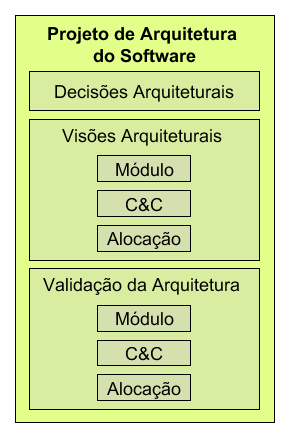
\includegraphics[width=0.32\textwidth]{projarquitect}
  \caption{Processos do Projeto de Arquitetura de Software} 
  \label{fig:projarquitect}
\end{figure}

%%%%%%%%%%%%%%%%%%%%%%%%%%%%%%%%%%%
%%%%%%%%%%%%%%%%%%%%%%%%%%%%%%%%%%%
\subsection{\textit{Decisões aquiteturais}}

Uma escolha entre as alternativas de design arquitetural, com o objetivo de atender um ou mais atributos de qualidade do sistema, são chamadas de decisões arquiteturais. Dessa forma, as decisões arquiteturais do MIDAS são descritas a seguir.

[Decisão Arquitetural 001] Mudança do uso de banco de dados para arquivo texto. Segundo os stakeholders a mudançã para arquivo texto faciliitou a comunicação e melhorou o desempenho do MIDAS.

[Decisão Arquitetural 002] Mudança do framework CodeIgniter para o Laravel. Por possuir uma grande comunidade de usuarios o grupo optou pela troca.
\textbf{ISSO ATENDE QUAL ATRIBUTO DE QUALIDADE?}

[Decisão Arquitetural 003] Mudança da plataforma de serviço para o Heroku, pelo motivo de o openshift provedor anterior, ter limitação na quantidade de colaboradores / desenvolvevores para trabalharem em um mesmo projeto. 



\subsection{\textit{Module View}}
\label{subsec:mv}
Um módulo é uma unidade de implementação de software que provê um conjunto de responsabilidades coerentes. Cada módulo possue uma coleção de propriedades associadas que expressam informações importantes (nome, visibilidade, restrições, etc).

Um módulo pode ser, por exemplo: 

\begin{itemize}
\item Pacote
\item Classe
\item Agrupamento geral de unidades de código
\end{itemize}

Para representar o MIDAS, foram utilizados o \textit{Decomposition Style}, o \textit{Data Model Style}, o \textit{Uses Style} e \textit{Layered Style}. 

\subsubsection{\textit{Decomposition Style}}

O \textit{Decomposition Style} é usado para dividir o sistema em unidades de implementação. Descreve a organização do código como módulos e sub-módulos e mostra como as responsabilidades do sistema são particionadas entre eles. Logo, na Figura ~\ref{decomposicao} é possível visualizar esse estilo do MIDAS.


\begin{figure} [h!]
  \centering
    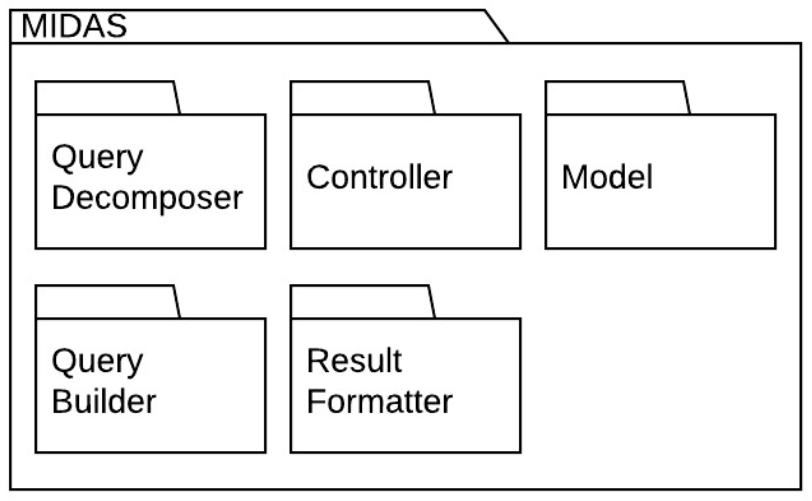
\includegraphics[width=0.7\textwidth]{MIDAS_-_Estilo_Decomposicao}
  \caption{MIDAS - \textit{Decomposition Style}}
  \label{decomposicao}
\end{figure}

\textbf{Módulo \textit{Controller}}

Responsável por receber do SAAS as requisições de consultas. Uma requisição de consulta contém informações que indicam o DAAS a ser acessado e os parâmetros da consulta (base de dados, ordenação, limite de registros recuperados, etc). 

Aciona o \textit{Query Decomposer} para a decomposição da requisição de consulta. Aciona o \textit{Query Builder} para a montagem da consulta a ser enviada ao DAAS. 

Executa uma consulta ao DAAS, recebe e encaminha o resultado da consulta para o \textit{Result Formatter}.

\textbf{Módulo \textit{Query Decomposer}}

Trata as requisições de consulta recebidas do \textit{Controller}, decompondo seus elementos (SELECT, FROM, WHERE, ORDER BY, LIMIT, etc.) e devolvendo a consulta decomposta. O \textit{Query Decomposer} é implementado como uma classe PHP.

\textbf{Módulo \textit{Query Builder}}

Recebe do \textit{Controller} a consulta decomposta por elementos e prepara uma consulta no formato aceito pelo DAAS de destino, de acordo com suas 
especificações de API REST - armazenadas no DIS. Devolve a consulta preparada ao \textit{Controller}. O \textit{Query Builder} é uma classe PHP.

\textbf{Módulo \textit{Model}}

Responsável por acessar as informações armazenadas no DIS (\textit{Dataset Information Storage}). O DIS guarda em arquivo texto informações relevantes de cada DAAS, como URL de conexão e informações de acesso à respectiva API REST. 

\textbf{Módulo \textit{Result Formatter}}

Classe PHP que recebe o resultado da consulta ao DAAS, juntamente com os parâmetros da requisição de consulta, através do \textit{Controller}. Pode receber os dados em formato JSON, CSV ou XML, a depender da API REST do DAAS. 
Filtra as informações e as organiza, de acordo com os parâmetros da requisição de consulta. Retorna ao \textit{Controller} os dados em formato JSON. 



\subsubsection{\textit{Data Model Style}}

O \textit{Data Model Style} descreve a estrutura da informação estática em termos de entidades de dados e seus relacionamentos. Ele facilita a comunicação com os \textit{stakeholders} durante a análise e elicitação de requisitos e guia a implementação das entidades em um banco de dados. O \textit{Data Model Style} do MIDAS é observado na Figura ~\ref{modelo}

\begin{figure} [h!]
  \centering
    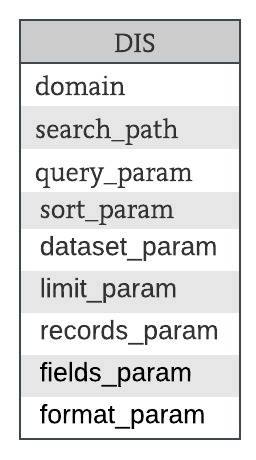
\includegraphics[width=0.3\textwidth]{MIDAS_-_Estilo_Modelo_Dados}
  \caption{MIDAS - \textit{Data Model Style}}
  \label{modelo}
\end{figure}

No MIDAS, conforme visto na Figura ~\ref{registro} os parâmetros que viabilizam o acesso ao DAAS ficam armazenados no DIS. O DIS é um arquivo texto e o seu conteúdo está no formato JSON. Optou-se pelo armazenamento em arquivo texto devido à simplicidade da estrutura e ao número reduzido de registros. 


\begin{figure} [h!]
  \centering
    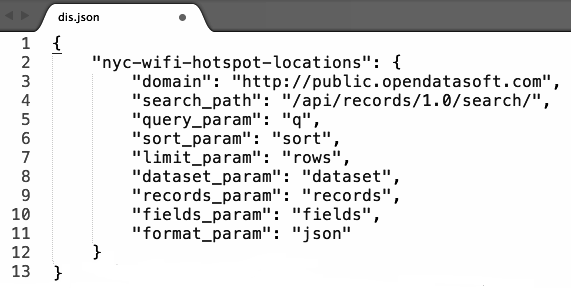
\includegraphics[width=0.7\textwidth]{DIS-exemplo}
  \caption{Exemplo de registro no DIS}
  \label{registro}
\end{figure}


\textbf{Atributos do DIS:}

\begin{itemize}
\item \textbf{domain: } domínio de hospedagem do DAAS, no formato URL \item \textbf{search path: } caminho de pesquisa para acessar os serviços do DAAS, complementa o domínio de hospedagem para a formação de uma consulta
\item \textbf{query param: } nome do parâmetro que identifica a query a ser executada no DAAS 
\item \textbf{sort param: } nome do parâmetro que identifica o critério de ordenação para a consulta ao DAAS
\item \textbf{limit param: } nome do parâmetro de identifica o critério de limite de registros a serem retornados pela consulta ao DAAS
\item \textbf{dataset param: } nome do parâmetro que identifica o dataset a ser consultado no DAAS 
\item \textbf{records param: } nome do parâmetro de retorno para identificar os registros retornados pelo DAAS
\item \textbf{fields param: } nome do parâmetro de retorno para identificar os campos retornados pelo DAAS
\item \textbf{format param: } formato do resultado da consulta ao DAAS
\end{itemize}



\subsubsection{\textit{Uses Style}}

O \textit{Uses Style} ilustra a dependência que pode existir entre dois módulos. Um módulo A usa B se a corretude de A depende da presença da correta implementação de B. 

\begin{figure} [h!]
  \centering
    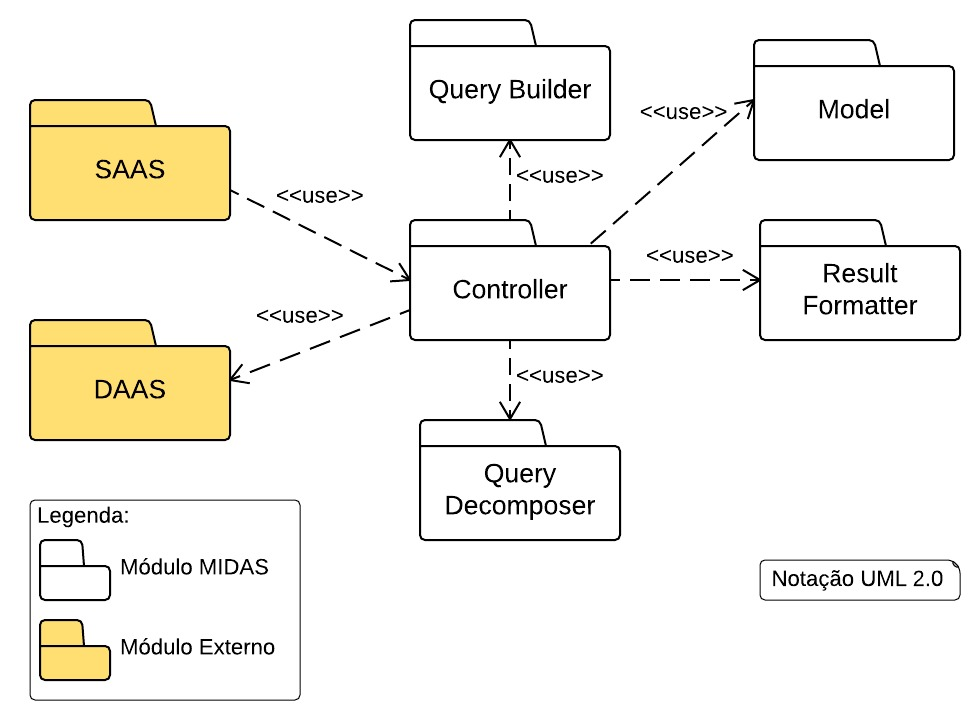
\includegraphics[width=0.9\textwidth]{MIDAS_-_Estilo_Uses}
  \caption{MIDAS - \textit{Uses Style}}
  \label{uses}
\end{figure}

Na \textit{Uses Style} representada na Figura ~\ref{uses}, o módulo \textit{Controller} aparece numa posição central, pois ele é quem requisita serviços aos outros módulos do MIDAS, assim como, recebe as requisições do SAAS e executa a consulta ao DAAS. 

O \textit{Controller} é quem inicia as comunicações com os outros módulos, recebendo uma resposta para as suas requisições. A única exceção é o SAAS, que é quem inicia a comunicação, sendo que o SAAS e o DAAS são módulos externos ao MIDAS. 


\subsubsection{\textit{Layered Style}}

Este estilo põe junto as camadas (agrupamento de módulos que oferecem um cojunto coesivo de serviços) em uma relação unidirecional "permitido para uso" entre as camadas.

Na figura ~\ref{camadas}, observa-se o SAAS, que é a camada externa ao MIDAS que inicia a comunicação. 

\begin{figure} [h!]
  \centering
    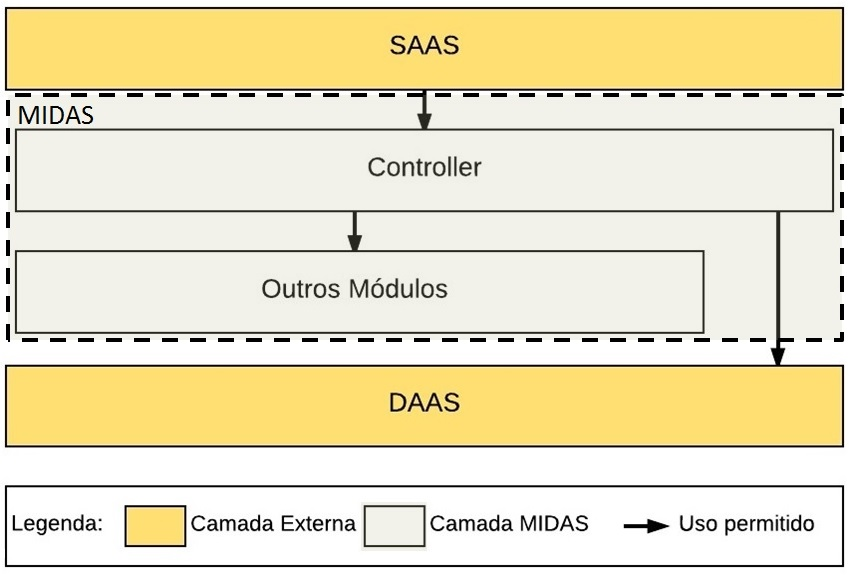
\includegraphics[width=0.8\textwidth]{MIDAS_-_Estilo_Camada}
  \caption{MIDAS - Estilo Camadas}
  \label{camadas}
\end{figure}

O tratamento da requisição do SAAS é feito pelo módulo \textit{Controller}, que é o responsável por orquestrar a comunicação interna do MIDAS, assim como, a comunicação com outros sistemas (SAAS e DAAS). Por isto, o módulo \textit{Controller} está representado como uma única camada isolada das demais. 

Os módulos \textit{Query Decomposer}, \textit{Query Builder}, \textit{Model} e \textit{Result Formater} formam uma outra camada do MIDAS. Estes módulos e não se comunicam diretamente. Todos eles são acionados pelo \textit{Controller} e somente respondem a este módulo após receberem uma requisição. 

O \textit{Controller} é o único módulo do sistema que se comunica com o DAAS. 

Este modelo proporciona um baixo acoplamento e uma alta coesão - isto é um direcionador do projeto MIDAS, visando uma maior facilidade de manutenção. 



%%%%%%%%%%%%%%%%%%%%%%%%%%%%%%%%%%%
%%%%%%%%%%%%%%%%%%%%%%%%%%%%%%%%%%%
\newpage

\subsection{Componente e conectores (C\&C)}
\label{subsec:cc}
Analisando o MIDAS sob a ótica da visão arquitetural de Componentes e Conectores, os módulos existentes correspondem a componentes. O estilo Cliente-Servidor foi utilizado para representar essa visão, conforme diagrama a seguir.

A descrição dos módulos e suas respectivas responsabilidades foram detalhados  anteriormente na visão de Módulo.

\begin{figure} [h!]
  \centering
    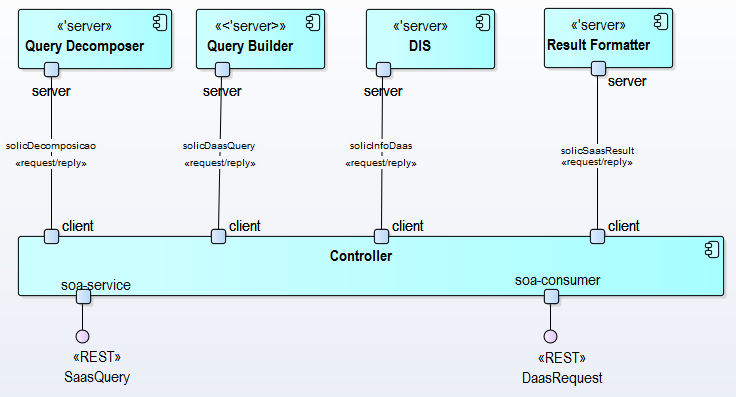
\includegraphics[width=0.8\textwidth]{MIDAS_-_Estilo_Cliente_Servidor}
  \caption{MIDAS - Estilo Cliente Servidor}
  \label{cliente}
\end{figure}

A diagramação utilizada na Figura ~\ref{cliente} obedece ao disposto na UML 2.0 com a adaptação de conectores feita em Clements Et Al \cite{clements2002documenting}, que não utiliza a montagem/assemby para representar os conectores e sim uma associação direta entre as portas.

No diagrama é possivel notar que existe um \textit{Controller} principal que é o que faz a conexão com todos os outros componentes do MIDAS. Nenhum componente acesso o outro diretamente que não seja através deste \textit{Controller}. O \textit{Controller} sempre chama os componentes mediante uma requisição de serviço, obtendo a resposta em seguida. Sendo assim, podemos considerar o \textit{Controller} como cliente de todos os outros componentes do MIDAS e todos os outros componentes como servidor do \textit{Controller}, utilizando o \textit{Component-and-Connector Style denominado  Client-Server} Clements Et Al \cite{clements2002documenting} para tal fim.

Os conectores possuem os papéis request e reply, para requisitar solicitações e responder solicitações, respectivamente. A porta \textit{client} está anexada ao papel request e a porta server está anexada ao papel \textit{reply} para os componentes dispostos, obedecendo ao definido por Clements Et Al \cite{clements2002documenting}.

O \textit{Controller}, além das portas clientes em relação aos outros componentes, ainda possui mais duas portas: uma para receber requisições SOA do SAAS e outra para comunicação com o DAAS, ambos através de conectores REST.


\newpage
%%%%%%%%%%%%%%%%%%%%%%%%%%%%%%%%%%%
%%%%%%%%%%%%%%%%%%%%%%%%%%%%%%%%%%%
\subsection{\textit{Allocation View}}\label{sec:aloc}
\label{subsec:av}
São representados na visão de alocação o \textit{Deployment Style} e o  \textit{Work Assignment Style}. O \textit{Implementation Style} não pôde ser documentado porque o acesso ao código-fonte não foi autorizado.

\subsubsection{Deployment Style}
O objetivo de utilizar o diagrama de implantação da UML é mapear os componentes e conectores no hardware onde o middleware é executado. O diagrama de implantação, abaixo, mostra quais são os componentes de hardware pensados na arquitetura do projeto, de que forma os componentes de software estão alocados e como essas diferentes peças se relacionam.

\begin{figure}[h!]
\centering
   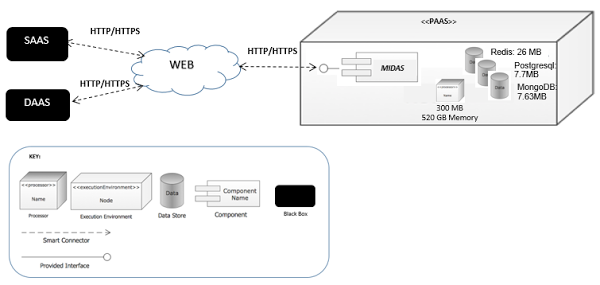
\includegraphics[width=0.95\textwidth]{MIDAS_-_Estilo_Deployment}
\caption{Diagrama de deployment}  \label{fig:deployment}
\end{figure}

Como mostra a Figura ~\ref{fig:deployment}, o MIDAS, que é totalmente desenvolvido em PHP, fica hospedado em um PaaS chamado HEROKU utilizando seu serviço de hospedagem de PHP e banco de dados, apesar de não pretender utilizar este último.

A versão do Heroku contratada é a “Free” que contempla a  configuração de hardware da Tabela~\ref{tab:hardware}

\begin{table}[h!]
\centering
\caption{Configuração de Hardware contratada} \label{tab:hardware}
\begin{tabular*}{0.7\linewidth}{@{\extracolsep{\fill}}|r p{7cm}|} \hline
\textbf{Disco} & 300 MB de armazenamento \\&520 GB de memória  \\ \hline
\textbf{ Banco de dados} & 
Redis
\begin{itemize}
\item versão: 3.2.4
\item memória: 278 KB de 26MB
\item conexões: 1 de 20
\end{itemize}
Postgresql
\begin{itemize}
\item versão 9.6.1
\item disco: 7.7 MB
\item registros: 336 de 10.000
\end{itemize}
MongoDB
\begin{itemize}
\item versão 3.2.11
\item disco: 7.63 MB
\item registros: 336 de 10.000
\end{itemize}
ClearDB
\begin{itemize}
\item disco: 0.08 MB de 5 MB
\end{itemize}
\\\hline
\textbf{Localização } & EUA \\ \textbf{do servidor}&\\\hline
\textbf{Software} & PHP versão 5.6 \\ 
& Framework Laravel versão 5.3 
  \\\hline
\end{tabular*}
\end{table}



A Plataforma HEROKU funciona executando aplicativos do cliente em contêineres virtuais que rodam em um ambiente de tempo de execução confiável. Quando o cliente necessita de uma máquina com PHP, que é o que ocorre com o MIDAS, o Heroku "imediatamente" a fornece, sendo indiferente para o cliente, qual será o SO do servidor com PHP.

Dessa forma, pelo fato de o MIDAS ser uma nuvem para aplicações, projetado para ser independente de infraestrutura, não cabe nesse projeto requisitar uma infraestrutura em específico. Se fosse determinado, por exemplo, que todo usuário deste middleware usasse o Windows com a justificativa de que o MIDAS foi feito pensando apenas neste SO, isso geraria um problema de lock-in para todos os usuários de MAC e Linux em uma solução que tenta justamente resolver esse problema.

\subsubsection{Work Assignment Style}

O objetivo deste estilo é descrever o mapeamento das pessoas que compõem a equipe com as tarefas para desenvolvimento do módulo. A Tabela~\ref{tab:was} mostra a organização dos elementos macro da estrutura de trabalho para desenvolver o MIDAS e respectivos executores.

\begin{table}[h!]
\centering
\caption{Work Assignment Style} \label{tab:was}
\begin{tabular*}{0.75\linewidth}{@{\extracolsep{\fill}}|r p{7cm}|} \hline
\textbf{Design} & Marcelo Aires, Elivaldo Lozer, Babacar Mane, Witã Rocha.  \\ \hline
\textbf{ Desenvolvimento} & Edmilson Lima, Joevan Santos.  \\\hline
\textbf{Teste} & Marcelo Aires, Elivaldo Lozer, Babacar Mane, Witã Rocha. \\\hline
\textbf{Gerente de projeto} & Daniela Claro
  \\\hline
\end{tabular*}
\end{table}

\newpage

%----------------------------------------------------------------------
\addcontentsline{toc}{section}{Refer\^{e}ncias} % Para incluir no sumário
\bibliographystyle{abbrv} %Mudar depois para abntex
\bibliography{references} % Nome do arquivo Bibtex (*.bib)


%----------------------------------------------------------------------
\appendix % a partir daqui todas as seções são tratadas como apendices
\newpage
\section{Um Ap\^{e}ndice}

Put your data here.

\subsection{Subseção}
Subseção.




%------------------------------------------------------------------------- 

\end{document}

 
